\documentclass{article}

%%%%
% PLOTS mapas y conglomerados
% bibliografia
%%%%
\usepackage[T1]{fontenc} %%%
\usepackage[utf8]{inputenc}
\usepackage{longtable}
\usepackage{authblk}
\usepackage{adjustbox}



\usepackage{natbib}

\title{LOS \'INDICES DE COLOMBIA}
% autores
\renewcommand\Authand{, y }
\author[1]{\normalsize MACQUEEN - SANTIAGO SERRANO}


\affil[1,2]{\small  Escuela de Ingenier\'ia,Universidad de los Andes\\
\texttt{{delcurso,deallado}@uniandes.edu.col}}
\affil[1]{\small Instituto de altas investigaciones financieras\\
Banco del Parque\\
\texttt{delcurso@bp.com.col}}

\date{30 de Junio de 2018}

%%%%
\usepackage{Sweave}
\begin{document}
\Sconcordance{concordance:FinaldeR3.tex:FinaldeR3.Rnw:%
1 29 1 1 0 25 1 1 13 4 1 1 6 15 0 1 3 11 1 1 10 1 2 9 1 1 17 1 6 15 1 1 %
4 12 0 1 3 3 1 1 14 13 0 1 2 6 1 1 4 1 3 13 1 1 6 1 4 31 0 1 2 10 1 1 %
75 8 1 1 17 1 3 11 1}


\maketitle


\begin{abstract}
El proposito principal de este trabajo es describir los procesos para partir una poblacion N-dimensional en partes de k tamano en forma de una muestra. El proceso, que se denomina 'k-means' aparece para dar particiones que son rasonablemente eficientes en el sentido de las variables dentro de las categorias. Eso es, que si p es la probabilidad de densidad para la poblacion S, S=s1,s2,...,Sn. La parte de En y de ui siendo i=1,2,3,..,k es el promedio condicional de p sobre S. Diremos de ahora en adelante en el documento 'tiende a ser bajo' para referirnos en principio a las consideraciones intuitivas y corroboradas del analisis matematico y practicas computacionales.
\end{abstract}

\section*{Introducci\'on}

The main purpose of this paper is to descrube a procces for partitioning an N-dimensional population into k sets on the basis of a sample. Th procvess, which is called 'k-means', appears to five partitions which are reasonably effcient in the sense of within-class variance. That is, if p is the probability mass functon for the population, S= S1,S2,..,Sn is a partition of En. We say 'tends to be low' primarily because of intutive considerations, corroborated to some extent by mthematical analysis and practical computational experience.


Comencemos viendo que hay en la secci\'on \ref{univariada} en la p\'agina \pageref{univariada}.

\clearpage



\section{Exploraci\'on Univariada}\label{univariada}

En esta secci\'on exploro cada \'indice. En esta secci\'on exploro cada \'indice. En esta secci\'on exploro cada \'indice. En esta secci\'on exploro cada \'indice. En esta secci\'on exploro cada \'indice. En esta secci\'on exploro cada \'indice. En esta secci\'on exploro cada \'indice. En esta secci\'`n exploro cada \'indice. En esta secci\'on exploro cada \'indice.


Para conocer el comportamiento de las variables se ha preparado  la Tabla \ref{stas} donde se describe la distribuci\'on de las modalidades de cada variable. Los n\'umeros representan la situaci\'on de algun pa\'is en ese indicador, donde el mayor valor num\'erico es la mejor situaci\'on.

	<<results=tex,echo=FALSE>>=
titulo <- "Tablas de estadisticos de regiones en Colombia"
vars1 <- colb[]
stargazer(vars1,title = "Medidas Estad<U+00ED>sticas", label = "Estad<U+00ED>sticas",summary.stat = c("n","mean","median","min","max"))

% Como apreciamos en la Tabla \ref{Tfrecuencias}, los pa\'ises en la mejor situaci\'on son los menos, salvo en el caso del \emph{\'indice de libertas mundial}\footnote{N\'otese que esto se puede deber a la {\bf menor} cantidad de categor\'ias.}

\clearpage

Para resaltar lo anterior, tenemos la Figura \ref{barplots} en la p\'agina \pageref{barplots}. 


%%%%% figure
\begin{figure}[h]
\centering

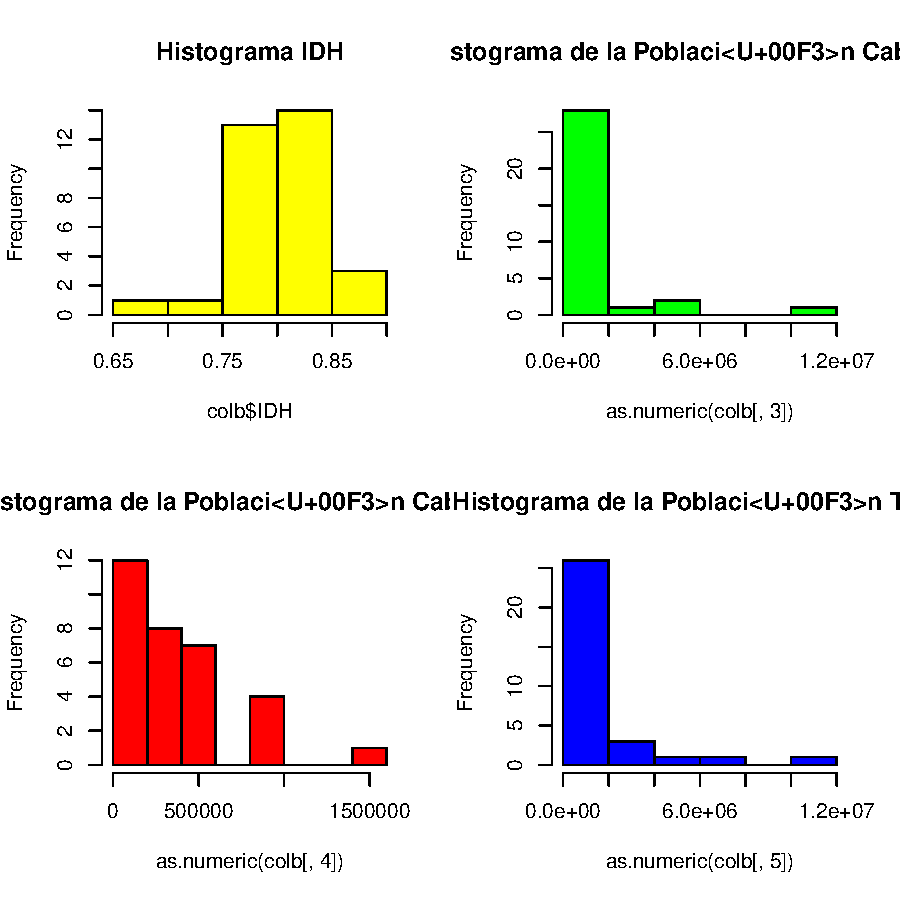
\includegraphics{FinaldeR3-barplots}


Debido al sesgo de las poblaciones sera necesario transformalas para que se acerquen a la normalidad y poder examinar bien.

\begin{adjustbox}{width=9cm,height=3cm,clip,trim=1.5cm 0.5cm 0cm 1.5cm}

	<<barplots, echo=FALSE,fig=TRUE>>=
col$cabeLog=log(as.numeric(colb[,3]))
col$cabeLog=log(as.numeric(colb[,4]))
col$cabeLog=log(as.numeric(colb[,5]))
par(mfrow=c(1,3))
###
title='Histograma de la Poblaci<U+00F3>n Cabecera'
paleta='green'
demoTableRelPlot=hist(as.numeric(colb[,7]),main=title,col=paleta)
###
title='Histograma de la Poblaci<U+00F3>n Cabecera'
paleta='red'
demoTableRelPlot=hist(as.numeric(colb[,8]),main=title,col=paleta)
###
title='Histograma de la Poblaci<U+00F3>n Total(Log)'
paleta='blue'
demoTableRelPlot=hist(as.numeric(colb[,9]),main=title,col=paleta)

\end{adjustbox}
\caption{Distribuci\'on de Indicadores}
\label{barplots}
\end{figure}
\clearpage


\section{Exploraci\'on Bivariada}

En este trabajo estamos interesados en el impacto de la poblaci\'on total en el IDH, veamos a contnuaci\'on el IDH con cada uno de ellos:

	<<corrDem, results=tex, echo=FALSE>>=
explanans=names(colb)[c(7:9)]
corrDem=cor(colb$IDH,colb[,explanans],
use = "na.or.complete")

stargazer(corrDem, title="Correlaci<U+00F3>n de Democracia con las dem<U+00E1>s variables",label = "corrDem")


Veamos la correlaci\'on entre las variables independientes:


	<<corrTablex, results=tex, echo=FALSE>>=
corrTableX=round(cor(colb[,explanans],
use = "na.or.complete"),2)
corrTableX_copy=corrTableX
corrTableX[upper.tri(corrTableX)]<-""
stargazer(corrTableX, title="Correlaci<U+00F3>n de Democracia con las dem<U+00E1>s variables",label = "corrTablex")

Lo visto en la Tabla \ref{corrTableX} se refuerza claramente en la Figura \ref{corrPlotX}.

\begin{figure}[h]
\centering
\begin{adjustbox}{width=7cm,height=7cm,clip,trim=1.5cm 0.5cm 0cm 1.5cm}

	<<verCorr, echo=false, fig=true>>=
plot(colb[,explanans], main = "Figura Logaritmos", ylab="Resto", xlab="Cabecera")

\end{adjustbox}
\caption{correlaci\'on entre predictores}
\label{corrPlotX}
\end{figure}


\clearpage

\section{Modelos de Regresi\'on}

Finalmente, vemos los modelos propuestos. Primero sin la libertad mundial como independiente, y luego con est\'a. Los resultados se muestran en la Tabla \ref{regresiones} de la p\'agina \pageref{regresiones}.

